\documentclass[a4paper,12pt]{article}
\usepackage[utf8x]{inputenc}
\usepackage{graphicx}   
\usepackage{amssymb,amsmath}
\usepackage{fancyheadings}
\usepackage{amsthm}
\usepackage{natbib}
\usepackage{enumerate}
\usepackage{algorithm}
\usepackage{subcaption}
\usepackage{lipsum}
\usepackage{algpseudocode}
\usepackage[margin=.8in]{geometry}
\usepackage{color}   %May be necessary if you want to color links
\usepackage{hyperref}
\hypersetup{
    colorlinks=true, %set true if you want colored links
    linktoc=all,     %set to all if you want both sections and subsections linked
    linkcolor=blue,  %choose some color if you want links to stand out
}

\lhead{Janitha Gunatilake}
\rhead{pFemView Documentation}
\title{pFemView: Documentation}
\author{Janitha Gunatilake}
\date{}

\begin{document}
\maketitle
%\tableofcontents
% \begin{abstract}
% \end{abstract}

\section{Introduction}
The open-source C++ library \emph{pFemView} enables visualizing $p$-hieararchical basis finite element solutions on the scientific visualization application ParaView \cite{parabook}.
As the VTK file format \cite{vtkBook} used in ParaView uses a linear or quadratic interpolation at specific geometric nodes, p-FEM solutions are not directly supported. Thus, additional work is required to visualize p-FEM solutions on ParaView effectively.
This library successfully bridges the $p$-FEM solutions and the ParaView application by generating a VTK file that can be directly read on ParaView. To do so, the user needs to input the p-FEM solution in the prescribed ``pFemView datafile format,'' which is discussed in detail in Section \ref{sec:pfv}.

\section{Overview of $p$-hierarchical basis finite element methods}

We refer to p-FEM originally proposed Babuska Szabo \cite{sb}, Rank Duster Axelsson Schwab Solin Pultarova
Gunatilake\cite{gunatilake2014, jg2022} serendipity space.

Beuchler and Korneev and Jensen uses a $p$-FEM method that is very similar, however using a tensor product space (instead of the serendipity space). In addition, the basis functions are scaled differently. Therefore, one cannot directly use pFemView to obtain VTK files for the $p$-FEM solutions. However, the concepts used here are applicable as well, and if needed one can easily modify the code to suit it.

\section{pFemView Datafile format}
\label{sec:pfv}
The legacy vtk file format to visualize p-hierarchical FEM solution comprises of five parts. 

\begin{enumerate}
\item \textbf{Header.} The header contains the single line: 
\begin{verbatim}
# vtk p-Hierarchical DataFile Version x.x
\end{verbatim}
This line must be exactly as shown with the exception of the version number x.x, which will vary with different
releases of VTK.
\item \textbf{Title.} The title consists of a character string terminated by end-of-line character \verb \n  and is 256 characters maximum. 
The title can be used to describe the data and include any other pertinent information.
\item \textbf{Data type.} The data type describes the type of file, either ASCII or binary. 
On\item \textbf{Geometry / Topology.} This part begins with a line containing the keyword DATASET followed by a keyword describing the type of dataset.
Then, depending upon the type of dataset, other keyword/data combinations define the actual data.
The cell types are indexed as follows.\\
0 - hexahedron\\
1 - tetrahedron\\
2 - wedge\\
3 - quadrilateral\\
4 - triangle\\
5 - line\\
\item  \textbf{Solution.} The final part describes the solution attributes. 
This part begins with the keyword \verb SOLUTION,  followed by an integer specifying the number of global degrees of freedom.
Other keyword/data combinations then define the actual dataset attribute
values (i.e., scalars, vectors, tensors, normals, texture coordinates, or field data).
The attribute \verb POLYNOMIAL_ORDERS , followed by an integer specifying the number of cells in the mesh, describes the polynomial order of each element. A 0-offset scheme is used.
Finally, the global dofs for each element are specified under the \verb GLOBAL_DOFS  attribute.
It is important to note that the global dofs must be numbered hierarchically. That means, all the vertices are added first. Then, the next modes are added in the order p is increased.
Having global dofs for $p-1$\textsuperscript{st} level assigned, the modes for pth level are added as follows.
First all the edge modes are added. Then all the face modes are added. If there are more than one face mode, first mode
is added to all faces before adding the second one and so on. Also quadrialeral faces are added before triangle faces. Finally all the interior modes are added.

\end{enumerate}

\section{Examples}
\subsection{A 2D Problem}
Following is a sample vtk file for hierarchical basis mesh with four quads ($2 \times 2$) and for polynomial order $p=2$. 

\begin{verbatim}
# vtk p-Hierarchical DataFile Version 3.0
AMR mesh
ASCII
DATASET UNSTRUCTURED_GRID
VERTICES 9 double
1 1 0
0 1 0
0.5 1 0
0 0 0
0.5 0 0
0.5 0.5 0
0 0.5 0
1 0 0
1 0.5 0

ELEMENTS 4
ELEMENT_TYPES 4
3
3
3
3
POLYNOMIAL_ORDERS 4
1
1
1
1
GLOBAL_DOFS 4
8 3 4 5 6 16 17 18 13 
8 4 7 8 5 12 14 19 17 
8 6 5 2 1 18 20 11 10 
8 5 8 0 2 19 15 9 20 

SOLUTION 21
SCALARS SolU double 1
LOOKUP_TABLE default
0
1.81547e-18
0
0
-7.51223e-19
0
0
0
0
0
-4.40983e-17
0
0
3.56351e-17
0
0
0
0
0
-1.81547e-18
0


\end{verbatim}

\subsection{A 3D Problem}
We solve
\begin{align*}
-\Delta u &= f \quad \text{ on } \Omega=(0,1)^3\\
u &= 0 \quad \text{ on } \partial \Omega
\end{align*}
where $f = 2yz(1-y)(1-z) + 2zx(1-z)(1-x) + 2xy(1-x)(1-y)$.
The exact solution to this boundary value problem:
\[
u_{\text{exact}} = xyz(1-x)(1-y)(1-z)
\]
Suppose we solve this problem via $p$-FEM on the following six-element tetrahedral mesh. 
\begin{figure}[h!]
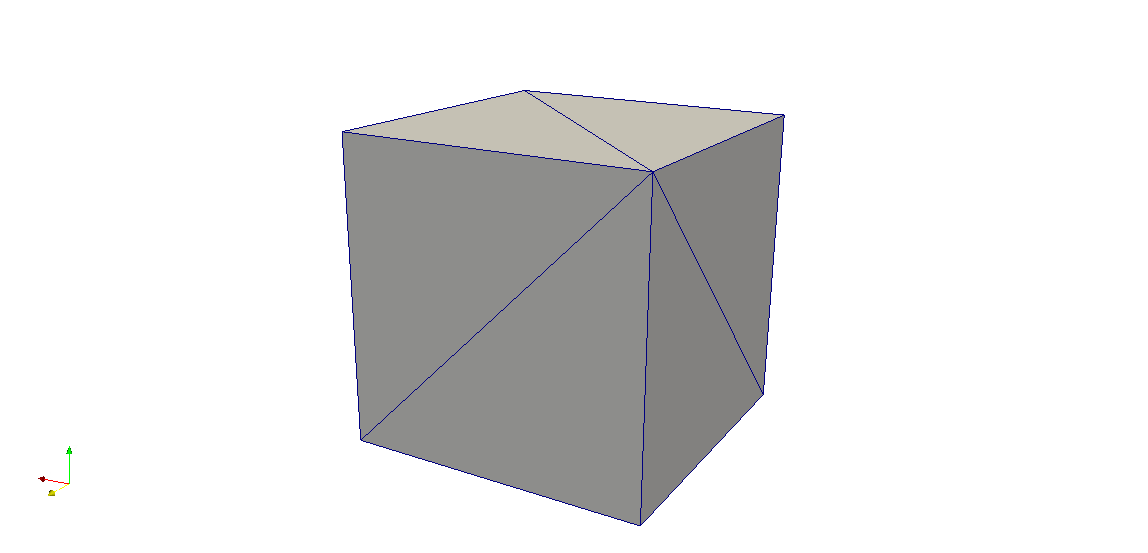
\includegraphics[scale=0.35]{tetCube.png}
\caption{ tetcube.}
\end{figure}

We will illustrate with a locally uniform p-refinement, and for simplicity, we use a finite element space with polynomial orders:
\[p=
\begin{cases}
2 & x<0.5,\\
3 & \text{otherwise.}
\end{cases}
\]
The pFemView datafile obtained solving the above problem with an iterative solver is shown below:
\begin{center}
\begin{verbatim}
# vtk p-hierarchical DataFile Version 3.0
AMR mesh
ASCII
DATASET UNSTRUCTURED_GRID
VERTICES 8 double
1 0 0
0 0 0
0 1 1
0 1 0
1 1 0
0 0 1
1 0 1
1 1 1
ELEMENTS 6 30
ELEMENT_TYPES 6
1
1
1
1
1
1
POLYNOMIAL_ORDERS 6
1
1
2
2
2
2
GLOBAL_DOFS 6
10 1 3 2 4 14 13 23 24 12 20 
10 0 2 1 5 22 23 10 21 17 9 
20 0 1 2 4 10 23 22 8 24 20 29 42 41 27 43 39 50 54 49 55 
20 0 2 5 6 22 17 21 11 25 16 41 36 40 30 44 35 51 56 57 58 
20 0 4 2 6 8 20 22 11 26 25 27 39 41 30 45 44 55 59 60 56 
20 2 6 4 7 25 26 20 19 18 15 44 45 39 38 37 34 60 61 62 63 

SOLUTION 64
SCALARS SolU double 1
LOOKUP_TABLE default
0
0
0
0
0
0
0
0
0
0
0
0
0
0
0
0
0
0
0
0
0
0
-0.0159083
0
0
0
0
0
0
0
0
0
0
0
0
0
0
0
0
0
0
0
0
0
0
0
0
0
0
0
0
0
0
0
0
0.075722
0.100234
0
0
0
0.223179
0
0
0
\end{verbatim}
\end{center}
\normalsize
The library pFemView reads this .pfv file, and generates a VTK file to be read by ParaView. This VTK file is quite large and could be accessed in the ``output'' directory named p3TetCube.vtk \url{https://github.com/janithag/pFemView/tree/main/output/p3TetCube.vtk}. Following is the plot of the solution obtained reading thie output VTK file on ParaView. We show a clip on the $x=0.5$ plane.
\begin{figure}[h!]
\centering
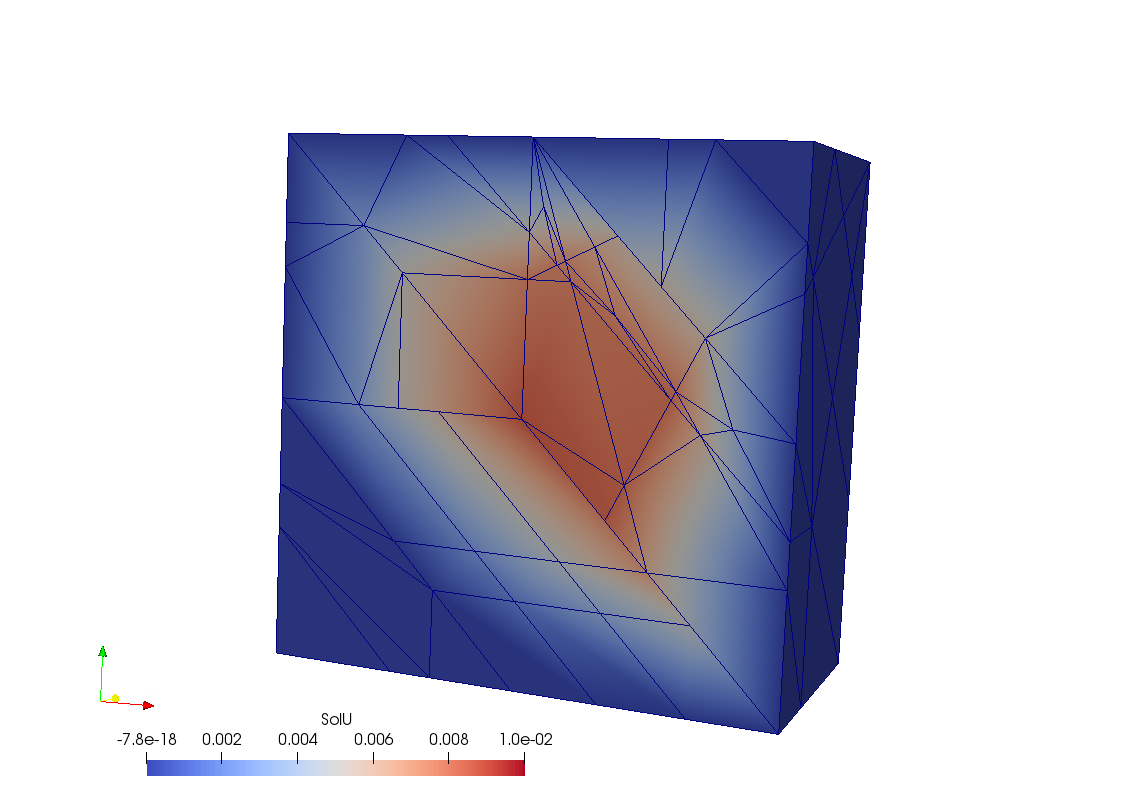
\includegraphics[scale=0.35]{tetCubeLocalPolyClipyEquals50d.png}
\caption{Local refinement p=2 if x<0.5 tetcube otherwise p=3. On the refined visualization mesh.}
\end{figure}

\bibliographystyle{plain}
\bibliography{references} 

\end{document}          
